%%\begin{figure}[htbp,width=0.9\textwidth]
%\begin{center}
%	\begin{tikzpicture}
%	\begin{axis}
%		[xmin=0,xmax=1,ymin=0,ymax=1,xtick={0,1},ytick={0,1},
%		xlabel=$x$,ylabel=$y$,title={Dominio fisico $\Oq$},
%		width=0.3\textwidth]
%	\end{axis}
%	\end{tikzpicture}
%	\hfill
%	\begin{tikzpicture}
%	\begin{axis}
%		[xmin=0,xmax=1,ymin=0,ymax=1,xtick={0,1},ytick={0,1},
%		xlabel=$x$,ylabel=$y$,title={Dominio di riferimento $\O$},
%		width=0.3\textwidth]
%	\end{axis}
%	\end{tikzpicture}
%\end{center}
%%\end{figure}
%%\\

%\begin{figure}
%	\begin{subfigure}
%		\includegraphics[draft=true]{Omegaq.jpg}
%		\caption{Dominio fisico $\Oq$}
%		\label{fig:Oq}
%	\end{subfigure}
%	\begin{subfigure}
%		\includegraphics[draft=true]{Omega0.jpg}
%		\caption{Dominio fisico $\O$}
%		\label{fig:O0}
%	\end{subfigure}
%\end{subfloat}

\begin{figure}[h]
	\centering
	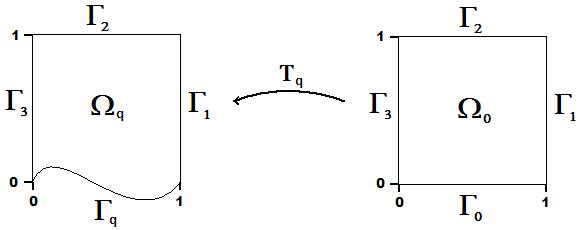
\includegraphics[width=0.7\textwidth]{Domini.jpg}
	\caption{Dominio fisico e dominio di riferimento}
\label{fig:domini}
\end{figure}